Все рассмотренные в предыдущем разделе методы перестроения поверхностей объединяет одно сходство -- они сохраняют количество элементов расчетной сетки (узлы, ребра, грани) и связи между ними.
Несмотря на некоторые специальные методы по предотвращению конфликтов между гранями сетки и методы сглаживания, после формирования новой поверхности возможно возникновение самопересечений, появление граней неправильной формы, а также неравномерное распределение граней в сетке по размеру.
Пока опустим самопересечения сетки и будем рассматривать только вопросы, касающиеся формы и размера ячеек.
Для определения качества формы ячейки треугольной формы с узлами $\vec{A}$, $\vec{B}$, $\vec{C}$ можно пользоваться простым критерием качества

\begin{equation}
Q(f) = \frac{4\sqrt{3} S_{ABC}}{|\vec{AB}|^2 + |\vec{BC}|^2 + |\vec{AC}|^2}
\end{equation}

где $Q(f) = 1$ соответствует идеальному случаю равносторонней ячейки, а $Q(f) = 0$ -- худший случай для ячеек с нулевой площадью \cite{Borouchaki}.

\begin{figure}
  \centering
  \begin{minipage}[h]{0.35\textwidth}
    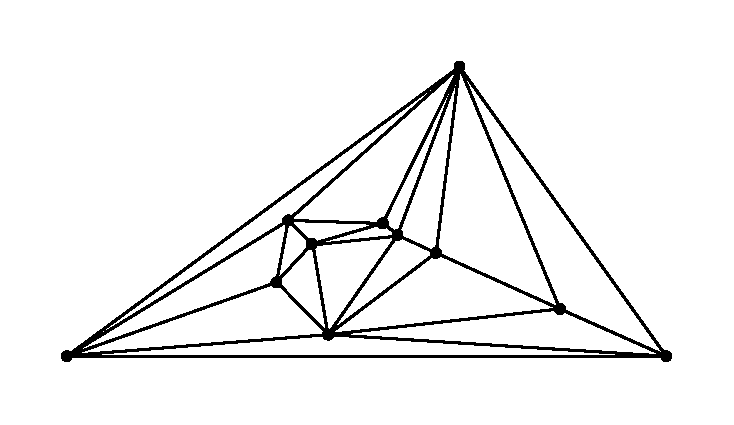
\includegraphics[width=\textwidth]{pics/pic_delaunay_size.pdf}
    \caption{Разбиение ячейки с помощью триангуляции Делоне.}\label{fig:pic_delaunay}
  \end{minipage}
  \hfill
  \begin{minipage}[h]{0.35\textwidth}
    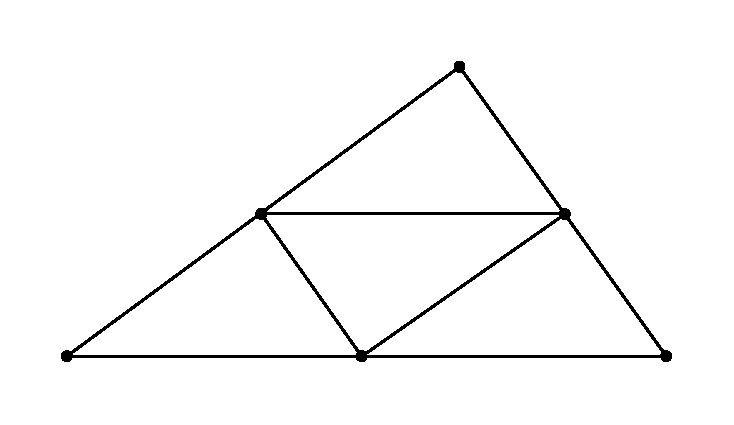
\includegraphics[width=\textwidth]{pics/pic_delaunay_2_size.pdf}
    \caption{Дробление ячейки на более мелкие.}\label{fig:pic_delaunay_2}
  \end{minipage}
  \hfill
  \begin{minipage}[h]{0.28\textwidth}
    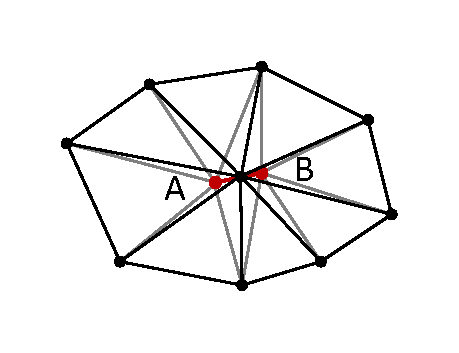
\includegraphics[width=\textwidth]{pics/pic_reduce_edge_size.pdf}
    \caption{Стягивание ребра.}\label{fig:pic_reduce_edge}
  \end{minipage}
\end{figure}
